\documentclass{article}

\usepackage[margin = 1in]{geometry}
\usepackage{amsmath}
\usepackage{amssymb}
\usepackage{graphicx,graphics}
\usepackage{float}


\title{Homework 1 \\ 
	\large COSC 522}
\author{Harshvardhan, Student ID: 609162}
\date{\today}

\begin{document}
	\maketitle


\section*{Problem 1}

\subsection*{Part 1}

Here are the normal curves drawn by hand using pencil and paper. Curve $A$ is $N(4,2)$, curve $B$ is $N(5,2)$ and curve $C$ is $N(6,3)$. (Please note that they are in different order than presented in the question.)

\begin{figure}[H]
	\centering
    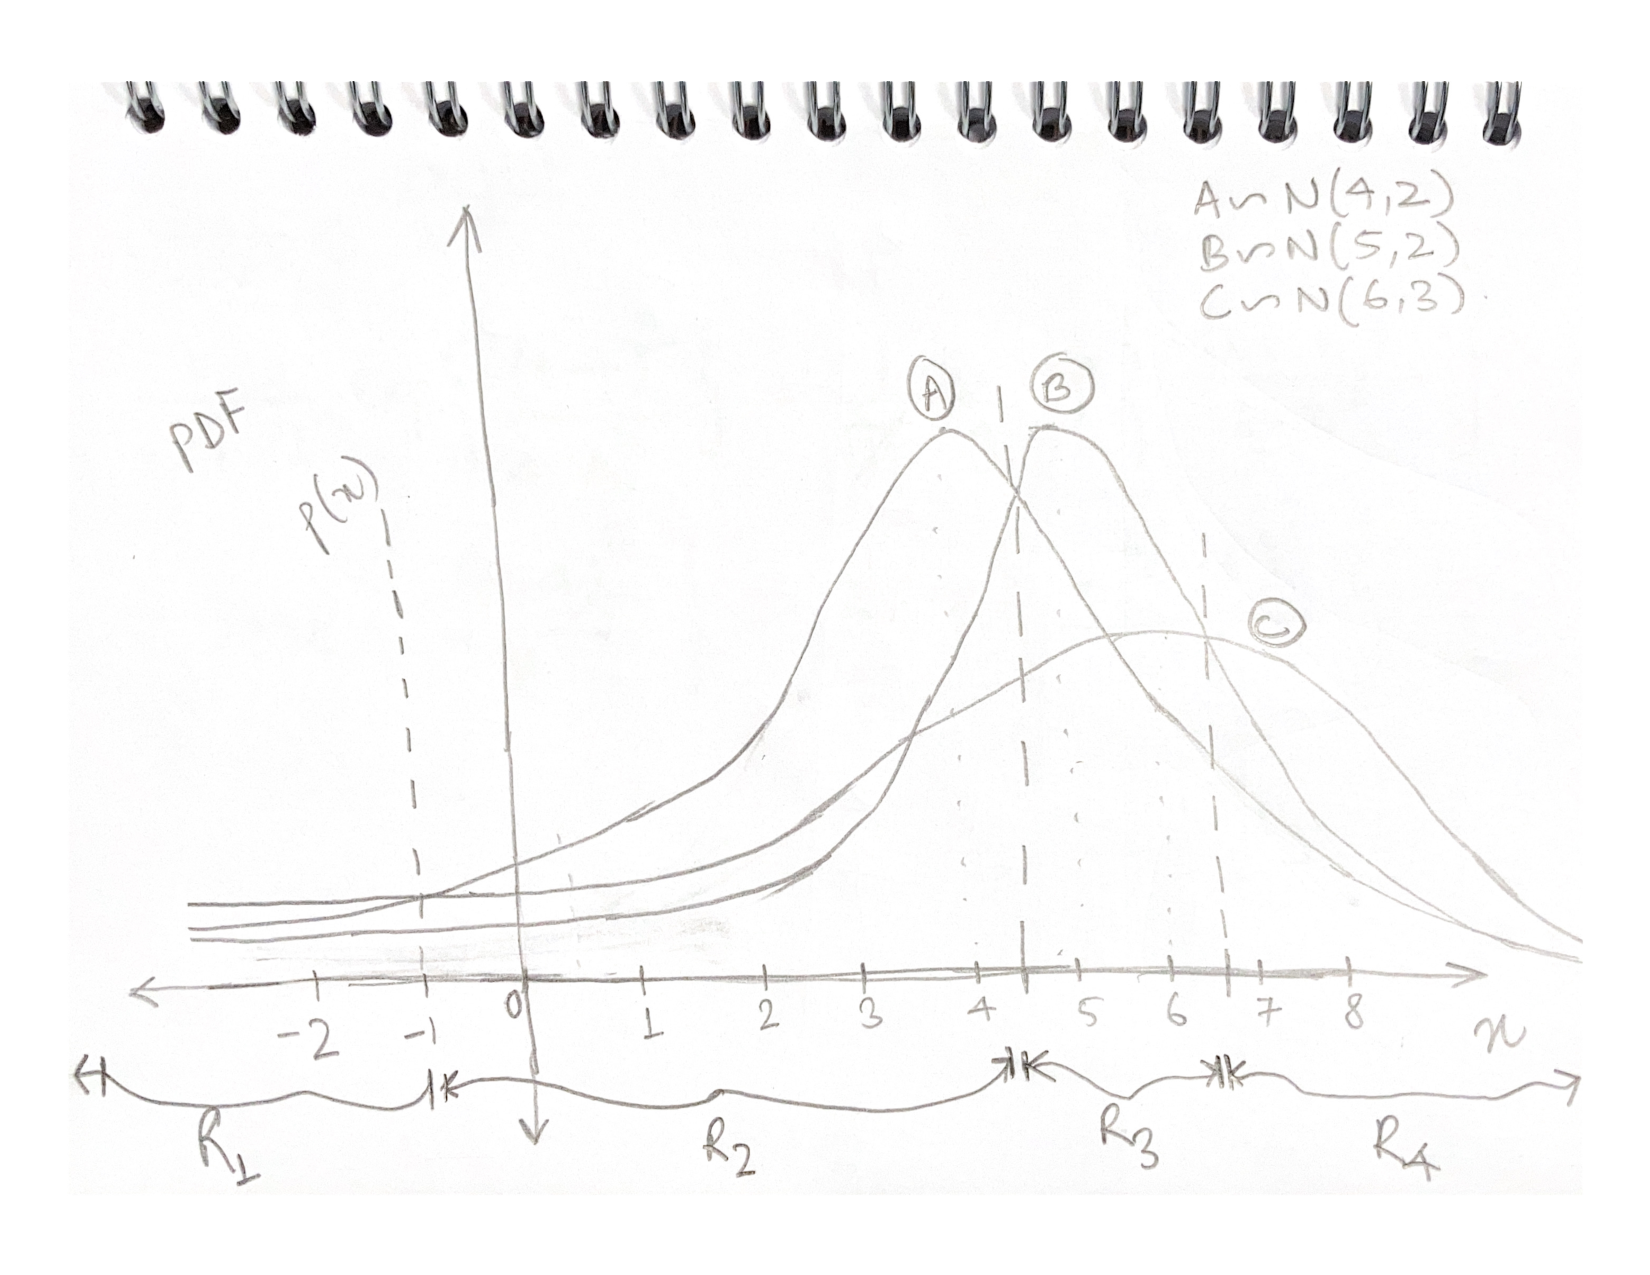
\includegraphics[width=\textwidth]{scan.pdf}
    \caption{Normal curves drawn with pencil. Please note that the labels $A$, $B$ and $C$ are in different order than presented in the question.}
    \label{fig:scan}
\end{figure}

Assuming equal prior probability, there would be three decision boundaries and consequently four decision regions. They are represented by $R_1$, $R_2$, $R_3$ and $R_4$ in figure \ref{fig:scan}.

\subsection*{Part 2}

\paragraph{(a)}

If $x = 4.7$, $P(w_i|x)$ is highest for $N(5,2)$. Therefore, it should be curve B in the figure \ref{fig:scan}, or the curve of $N(5,2)$. Curves $A$ and $B$ cross exactly at $4.5$.

To find this analytically, we will find the density of each curve at $x=4.7$. Whichever has the highest density, $x=4.7$ will belong to that class.

For $A$, density is 0.1876202. For $B$, density is $0.1972397$. For $C$, density is $0.1210635$. (All found using calculator.) So, it should be in curve B which is distributed as $N(5,2)$. The results are the same as from the graphical method.

\paragraph{(b)}

To find the exact decision boundaries, we will have to find the intersection points between the curves.

In the figure above, it is clear that the first boundary between $R_1$ and $R_2$ is the intersection between the curves represented by $A$ and $C$. Finding the intersection point:

$$
\frac{1}{2\sqrt{2\pi}} \exp{\frac{-(x-4)^2}{2 \times 2^2}} = 
\frac{1}{3\sqrt{2\pi}} \exp{\frac{-(x-6)^2}{2 \times 3^2}}
$$

$$
\implies
3\times \exp{\frac{-(x-4)^2}{8}} = 
2\times \exp{\frac{-(x-6)^2}{18}}
$$

Taking natural logarithm both sides,

$$
\implies
\ln{3} - \frac{(x-4)^2}{8} = 
\ln{2} - \frac{(x-6)^2}{18}
$$

$$
\implies \frac{(x-6)^2}{18} - \frac{(x-4)^2}{8}
 = \ln{2} - \ln{3}
$$


$$
\implies \frac{4(x-6)^2 - 9(x-4)^2}{72} = \ln{2} - \ln{3}
$$

$$
\implies \frac{4x^2 + 144 - 48x - 9x^2 - 144 + 72x}{72} = \ln{2} - \ln{3}
$$

$$
\implies -5x^2 + 24x = 72(\ln{2} - \ln{3})
$$

Using Sridharacharya rule,
$$
x = \frac{24 \pm \sqrt{24^2 - 4\times5\times72(\ln{2} - \ln{3})}}{10},
$$

That is, $x = -1.0056$ or $x = 5.805$. Since we are looking at $x<0$, the decision boundary is at $x = -1.0056$.

The second boundary is the intersection between the curves $A$ and $B$. Finding the intersection point:

$$
\frac{1}{2\sqrt{2\pi}} \exp{\frac{-(x - 4)^2}{2\times 2^2}} = 
\frac{1}{2\sqrt{2\pi}} \exp{\frac{-(x - 5)^2}{2\times 2^2}}
$$

$$
\implies (x-5)^2 = (x-4)^2
$$

$$
\implies (x-5-x+4)(x-5+x-4) = 0
$$

$$
\implies x = 9/2 = 4.5
$$

There is only one intersection point. Therefore the second boundary line is at $x = 4.5$. 

The third decision boundary is at the intersection of curves $B$ and $C$.

$$
\frac{1}{2\sqrt{2\pi}} \exp{\frac{-(x - 5)^2}{2\times 2^2}} = 
\frac{1}{3\sqrt{2\pi}} \exp{\frac{-(x - 6)^2}{2\times 3^2}}
$$

$$
2 \times \exp{\frac{-(x - 6)^2}{2\times 3^2}} = 
3 \times \exp{\frac{-(x - 5)^2}{2\times 2^2}}
$$

Taking natural logarithm both sides, 

$$
\ln{2} - \frac{(x - 6)^2}{18} = 
\ln{3} - \frac{(x - 5)^2}{8}
$$

$$
\implies \frac{(x - 5)^2}{8} - \frac{(x - 6)^2}{18} = \ln{3} - \ln{2}
$$

$$
\implies \frac{9(x-5)^2 - 4(x-6)^2}{72} = \ln{3} - \ln{2}
$$

$$
\implies
9x^2+225-90x-4x^2-144+48x=72(\ln{3} -\ln{2})
$$

By Sridharacharya Rule,

$$
x = \frac{42\pm\sqrt{42^2 - 4\times5\times72(\ln{3}-\ln{2})}}{10}
$$

So, $x = 6.897906$ or $x = 1.502094$. By visual inspection, we have to find $x$ that is between 6 and 7. Thus, the third decision boundary is at $x=6.897906$.

To conclude, here are our decision boundaries from left to right are the following: $x =  -1.0056,\; 4.5, \;6.8979$. Please note that these solutions were calculated using a calculator and only first few significant digits are shown.

\paragraph{(c)}

The overall probability of error is:

$$
P(error) =
\int_{-\infty}^\infty P(error|x)p(x) dx
$$

$$
= \int_{R_1} P(e_1|x)p(x) dx + \int_{R_2} P(e_2|x)p(x) dx + 
\int_{R_3} P(e_3|x)p(x) dx + \int_{R_4} P(e_4|x)p(x) dx
$$

Assuming equal prior probability ($=1/3$),

\begin{multline*}
=(
\int_{-\infty}^{-1.0056} f_{4,2}(x) dx + \int_{-\infty}^{-1.0056} f_{5,2}(x) dx + \int_{-1.0056}^{1.502}f_{6,3}(x) dx +  \int_{-1.0056}^{1.502}f_{5,2}(x) dx \;+ \\
\int_{1.502}^{4.5} f_{5,2}(x) dx + \int_{1.502}^{4.5} f_{6,3}(x) dx + \int_{4.5}^{5.805} f_{4,2}(x) dx + \int_{4.5}^{5.805} f_{6,3}(x) dx \;+ \\
 \int_{5.805}^{6.898} f_{6,3}(x) dx + \int_{5.805}^{6.898} f_{4,2}(x) dx + \int_{6.897}^{\infty} f_{5,2}(x) dx + \int_{6.897}^{\infty} f_{4,2}(x) dx
 ) \times \frac{1}{3}
\end{multline*}

\begin{multline*}
= (
(F_{4,2}(-1.0056) + F_{5,2}(-1.0056) + F_{6,3}(1.502) - F_{6,3}(-1.0056) + F_{5,2}(1.502) - F_{5,2}(-1.0056) \; + \\
F_{5,2}(4.5) - F_{5,2}(1.502) + F_{6,3}(4.5) - F_{6,3}(1.502) + F_{4,2}(5.805) - F_{4,2}(4.5) + F_{6,3}(5.805) - F_{6,3}(4.5) \; + \\
+ F_{6,3}(6.898) - F_{6,3}(5.805) + F_{4,2}(6.898) - F_{4,2}(5.805) + 1 - F_{5,2}(6.987) + 1 - F_{4,2}(6.987)
)/3
\end{multline*}

$$
= 1.570856 / 3 = 0.5236187,
$$

which is high. This is possible because the curves have huge overlaps.

\subsubsection*{Part 3}

\paragraph{(a)}

It is given that $P(w_1) = 0.6$, $P(w_2) = 0.2$ and $P(w_3) = 0.2$. Posterior probability is proportional to the product of prior probability and likelihood. Therefore,

$$
P(w_i|x) \propto p(x|w_i) \times p(w_i).
$$

The posterior probability plot is below (ignoring $p(x)$ as it is a constant).

\begin{figure}[H]
	\centering
    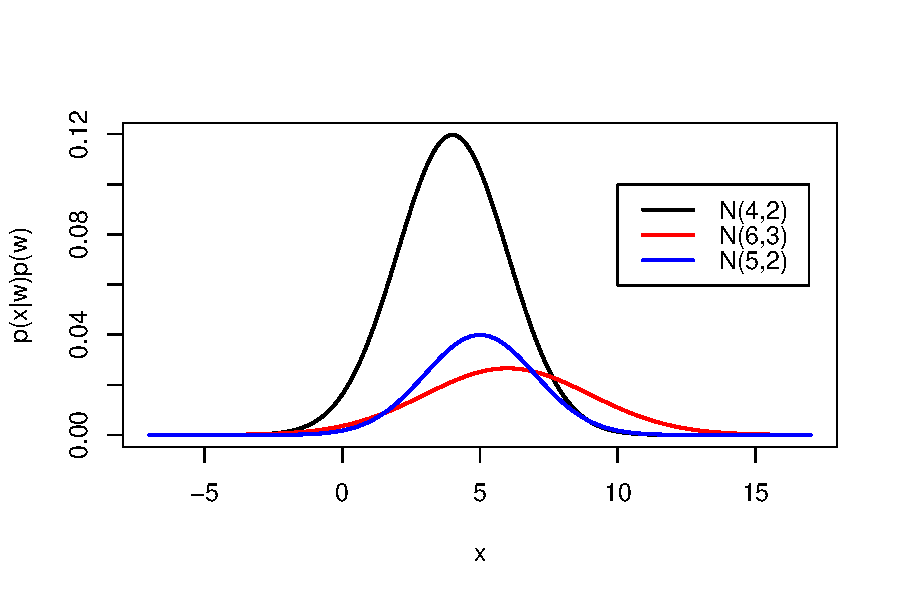
\includegraphics[width=\textwidth]{Rplot01.pdf}
    \caption{Posterior probability plots drawn using R.}
    \label{fig:plot1}
\end{figure}

\paragraph{(b)}

Following from 2(a), probability for each class will be product of posterior probability and likelihood.

For $A$, density is $0.1876202 \times 0.6 = 0.1125721$. For $B$, density is $0.1972397 \times 0.2 = 0.03944793$. For $C$, density is $0.1210635 \times 0.2 = 0.02421271$. (All found using calculator.) So, it should be in curve A which is distributed as $N(4,2)$. The results are the same as from the graphical method as the black curve has the highest density for $x = 4.7$.


\section*{Problem 2}

Actual positive belong in class 2. Actual negative belong in class 1.

\subsection*{Part 1}

PDF of $U(0,1)$ is 1 for all $x \in [0,1]$. PDF of $U(0.95,3.95)$ is $1/3$ for all $x \in [0.95, 3.95]$.

\begin{figure}[H]
	\centering
    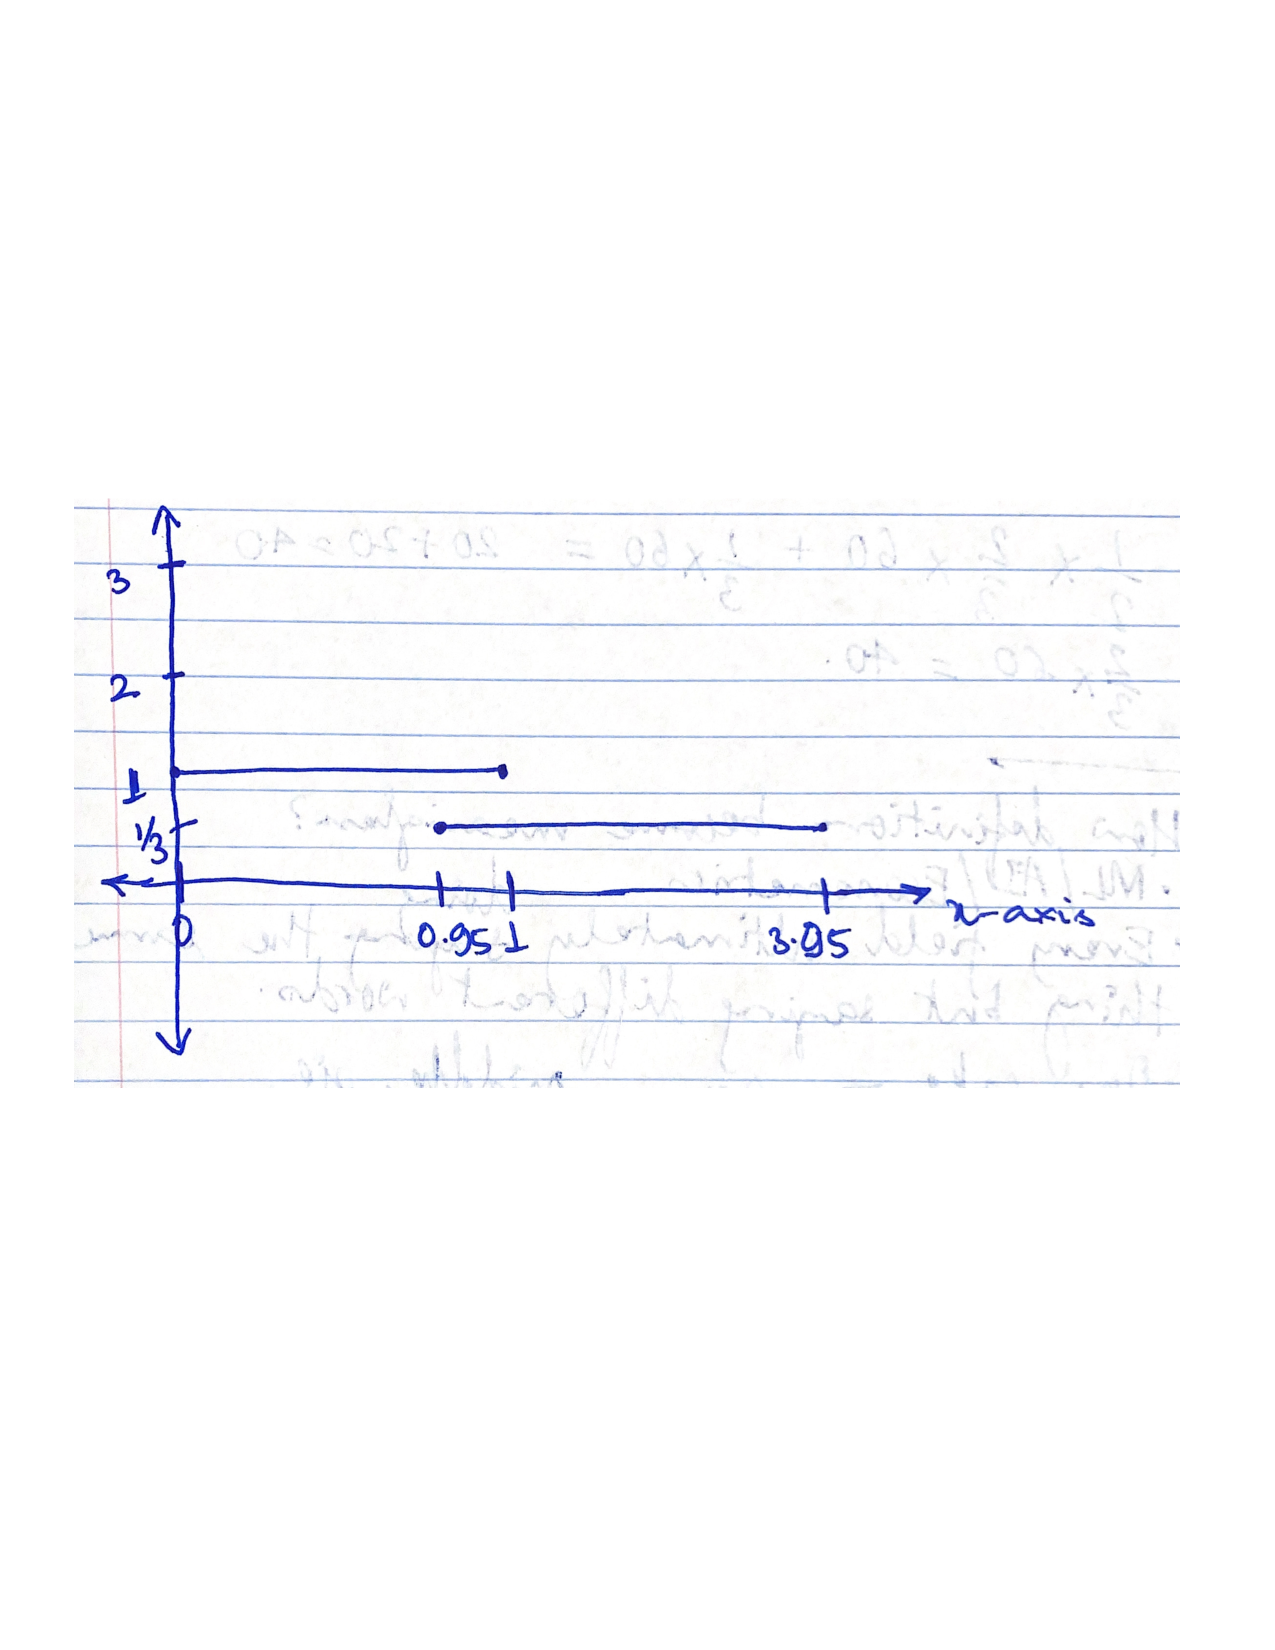
\includegraphics[width=\textwidth]{part2a.pdf}
    \caption{Uniform distribution plots drawn by hand.}
    \label{fig:plot3}
\end{figure}

\subsection*{Part 2}

We choose the decision boundary of 0.97. So, our figure becomes the following.

\begin{figure}[H]
	\centering
    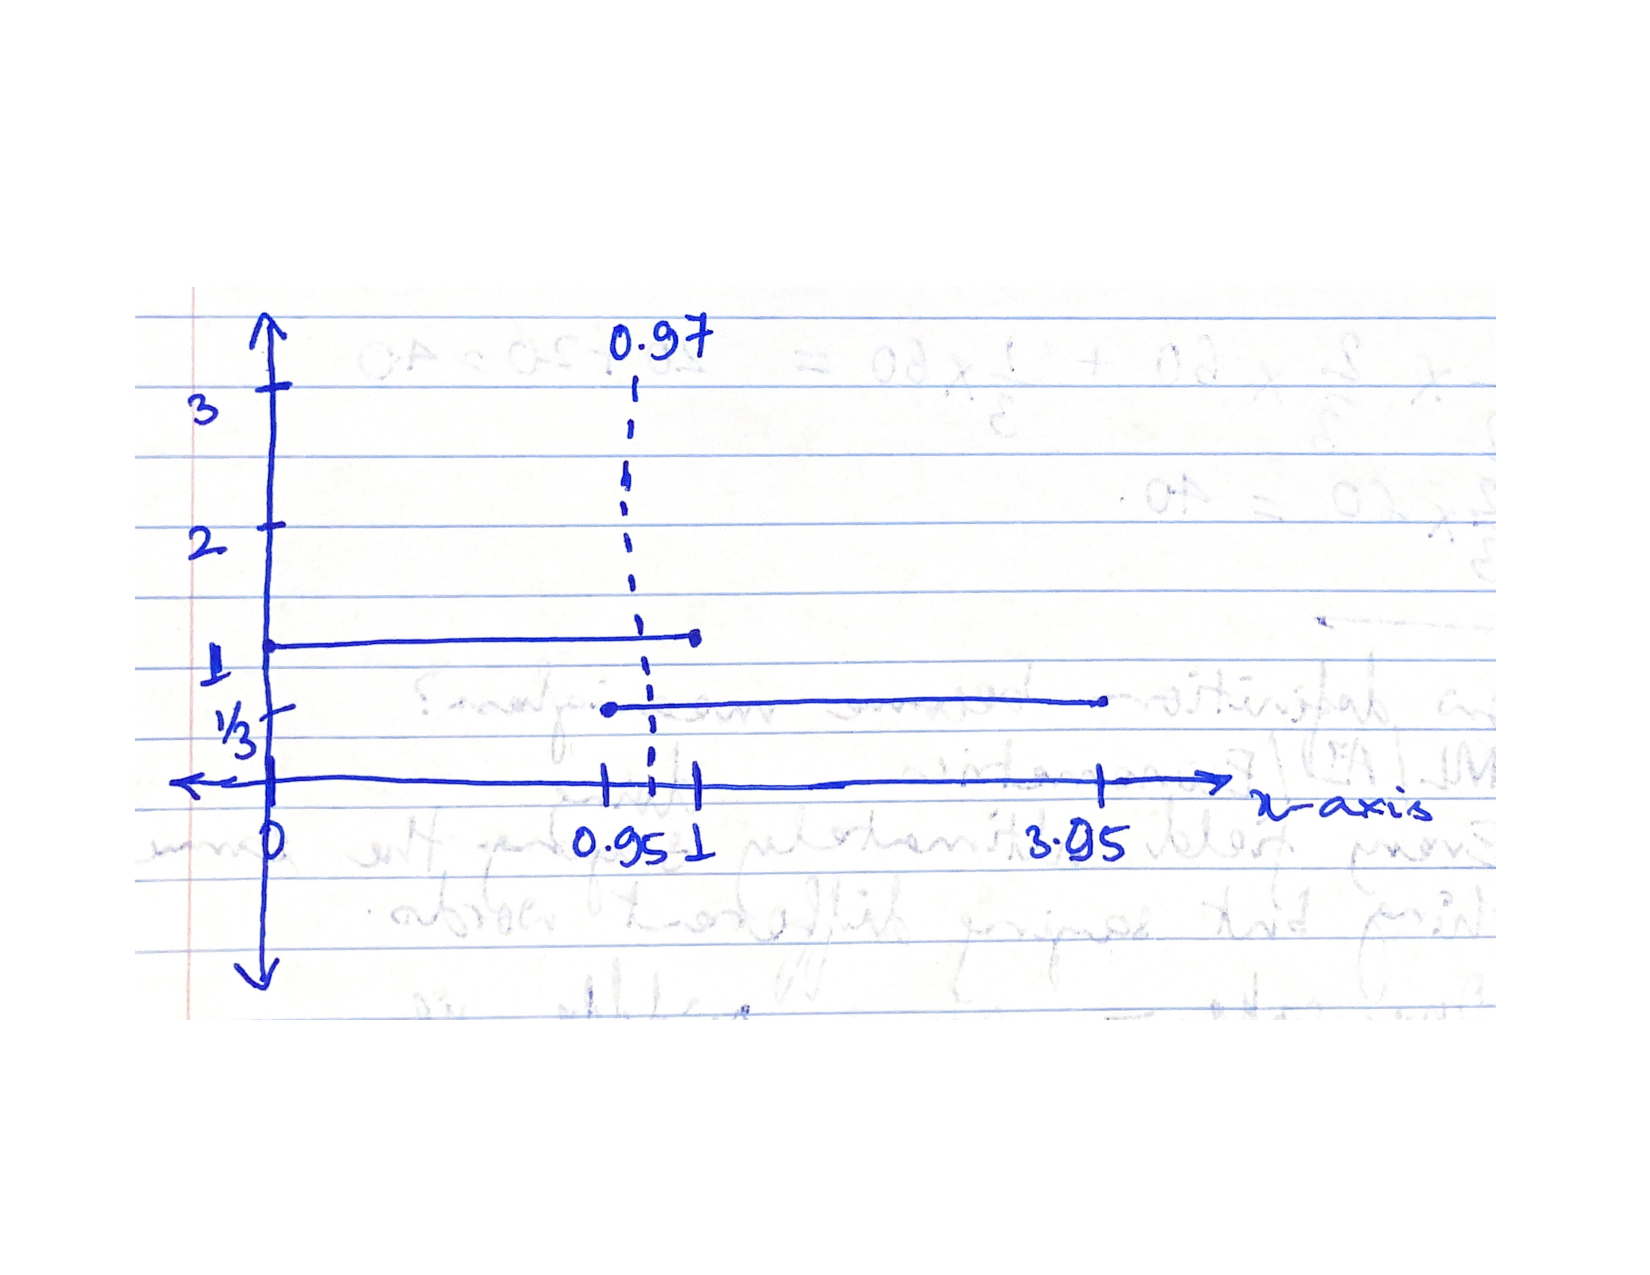
\includegraphics[width=\textwidth]{plot4.pdf}
    \caption{Uniform distribution plots drawn by hand with decision boundary at 0.97.}
    \label{fig:plot4}
\end{figure}

All with $x>0.97$ will be classified as positive and others will be classified as negative.

\paragraph{(a)} 

False-negative will be the cases when $0.95<x<0.97$. Calculating the same for continuous probability distribution (assuming equal prior probability of 0.5), we get:

$$
P(FN) = 0.5 \times P(0.95<x<0.97 | x \sim U(0.95, 3.95)) = 0.5(F(0.97) - F(0.95))
$$

$$
\implies P(FN) = 0.5 \times \frac{0.97-0.95}{3.95-0.95} = 0.02/3*0.5 = 0.003333 = 0.33\%.
$$

So, probability of false-negative is 0.33\%.

\paragraph{(b)}
False positive will be the cases when $0.97<x<1$. Calculating the same for continuous probability distribution (assuming equal prior probability of 0.5), we get:

$$
P(FP) = 0.5 \times P(0.97<x<1 | x \sim U(0,1)) = 0.5(F(1) - F(0.97))
$$

$$
\implies P(FP) = 0.5 \times \frac{1-0.97}{1} = 0.015 = 1.5\%.
$$

So, probability of false-positive is 1.5\%.

\paragraph{Note} I have assumed the prior probability of 0.5 (i.e. equal prior probability) as it wasn't mentioned in question what value to use. However, realistically speaking, \textit{any} disease will likely have a prior probability of much lower than 50\%, say in the ball park of 5 to 10\%.


\subsection*{Part 3}

We have to find the optimal decision boundary that minimises the overall probability of error. 

\begin{figure}[H]
	\centering
    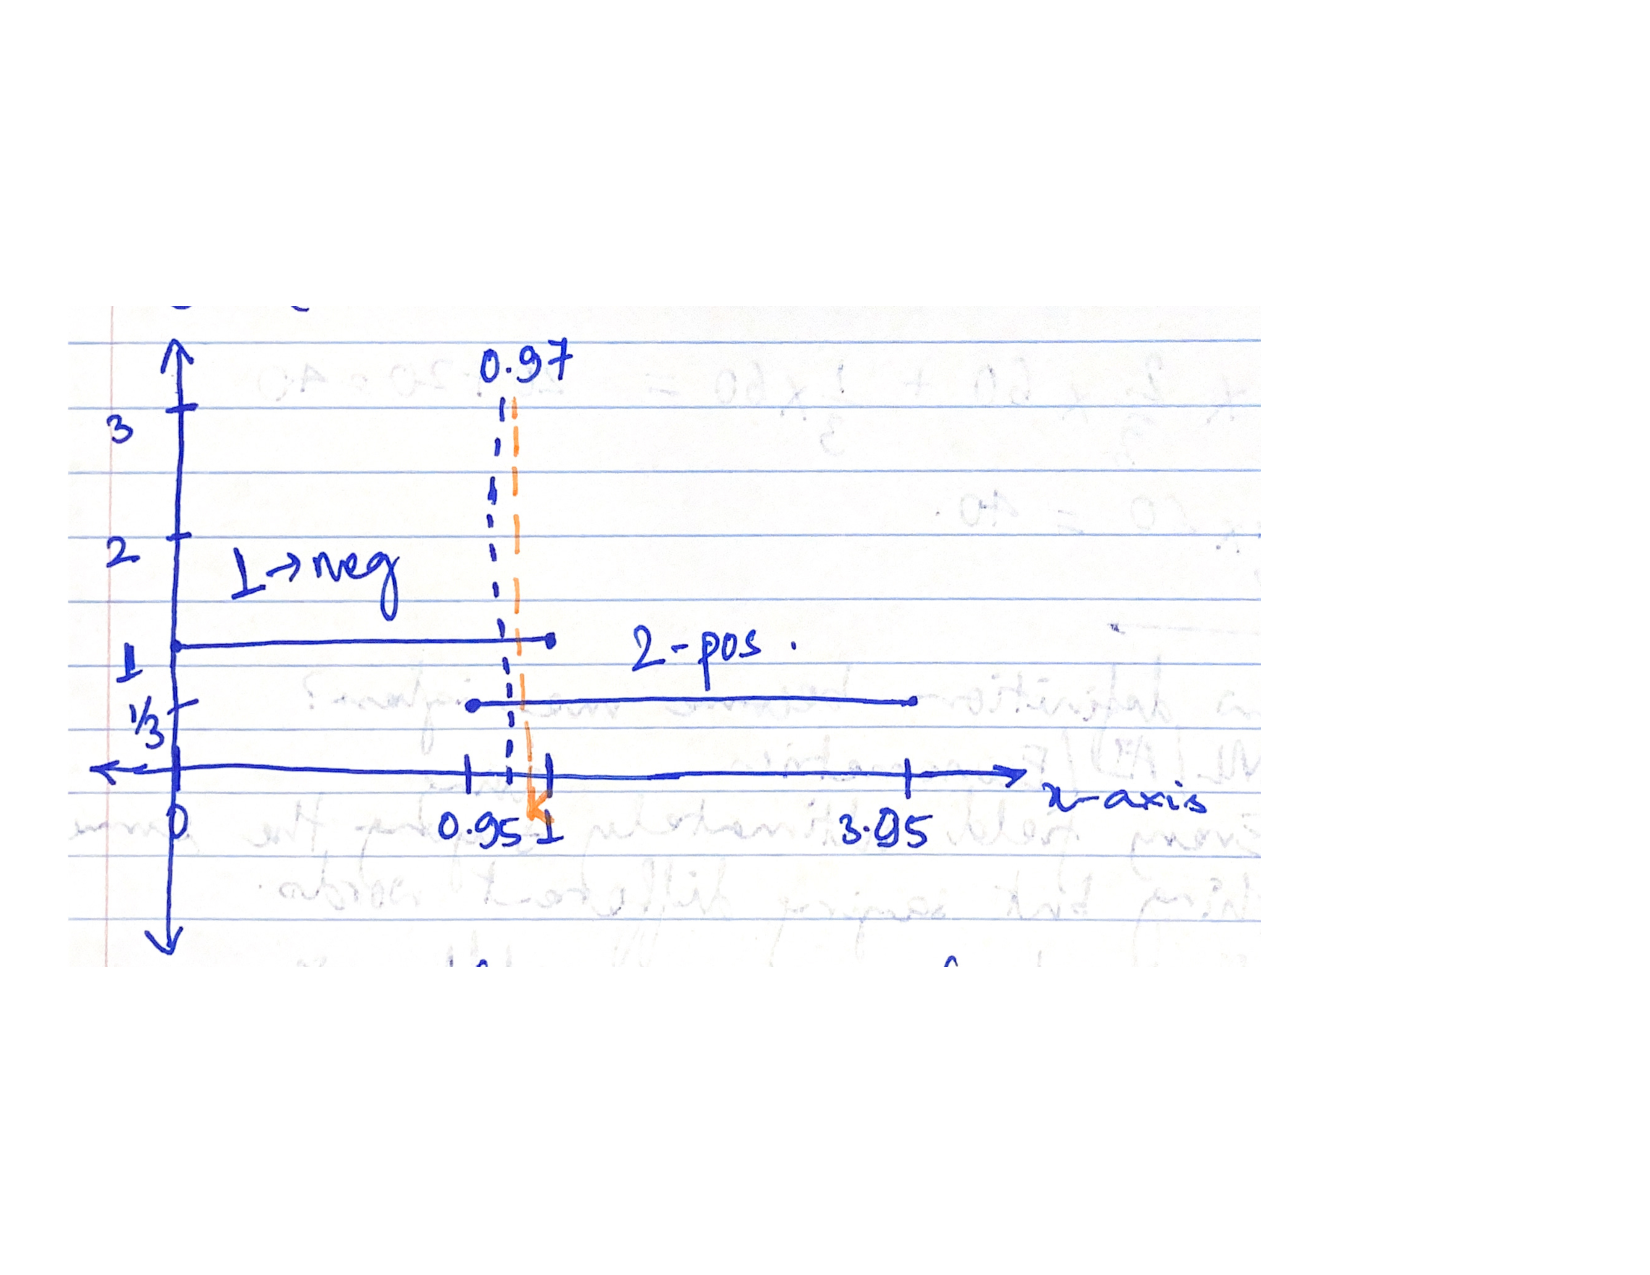
\includegraphics[width=\textwidth]{plot5.pdf}
    \caption{Uniform distribution plots drawn by hand with decision boundary at 0.97 and $k$. Decision boundary at $k$ is represented with orange dashed line.}
    \label{fig:plot5}
\end{figure}

The figure representing the boundary $k$ is shown in orange colour in the figure \ref{fig:plot5}. 

If $k$ is the optimal decision boundary, the area under the curves at that point should be equal for both the classes. That is,

$$
(k-0.95)\times\frac{1}{3} \times 0.5 = (1-k)\times1 \times 0.5,
$$

as both areas are rectangles. 

Therefore, solving the above equation would give the optimal boundary.

$$
\implies k - 0.95 = 3-3k
$$

$$
\implies k = 3.95/4 = 0.9875.
$$

So the optimal decision boundary is at $x = 0.9875$, assuming equal prior probability of 0.5. Therefore, 0.97 is the not the optimal decision boundary in Bayesian sense.

For $x=0.9875$ and equal prior probability, the probability of error is 

$$
(0.9875-0.95)\times\frac{1}{3} \times 0.5 + (1-0.9875)\times1 \times 0.5 = 0.0125 = 1.25\%.
$$

Consider the case that equal prior probability is not assumed and the prior probabilities are say $m$ and $1-m$. We have to find the value of $m$ for which the following expression is minimum:
$$
(0.9875-0.95)\times \frac{1}{3} \times m + (1-0.9875) \times (1-m).
$$

This expression is equal to $1$. Thus we conclude that for any value of $m$, this is the lowest error value that we can achieve; the error value doesn't depend on prior probabilities.

%We have to minimise

%$$
%P(error) = \int_{0.95}^k p(w_1|x \sim U(0.95, 3.95)) 0.5 dx + \int_{k}^1 p(w_2|x \sim U(0,1)) 0.5 dx,
%$$
%
%$$
%P(error) = \int_{0.95}^k \frac{x-0.95}{3.95-0.95} 0.5 dx +\int_k^1 \frac{x-0}{1-0} 0.5 dx
%$$
%
%$$
%P(error) = \int_{0.95}^k \frac{x-0.95}{6} dx +\int_k^1 \frac{x}{2} dx
%$$
%
%$$
%P(error) = 
%\left[ 
%\frac{x^2}{12} - \frac{0.95x}{6}
%\right]_{0.95}^k +
%\left[
%\frac{x^2}{4}
%\right]_k^1
%$$
%
%$$
%P(error) = \frac{k^2}{12} - \frac{0.95k}{6} - \frac{0.95^2}{12} + \frac{0.95^2}{6} + \frac{1}{4} - \frac{k^2}{4} = g(k)
%$$
%
%Differentiating $g(k)$ with respect to $k$ to minimise the probability of errors, we get:
%
%$$
%\frac{d \;g(k)}{dk} = \frac{k}{6} - \frac{0.95}{6} - \frac{k}{2}.
%$$
%
%Setting this to zero, 
%
%$$
%
%$$





































\end{document}